\documentclass[12pt,oneside,abbrevs,dtc,mscres,neuro,notimes,logo]{styles/infthesis}

\usepackage{reportpackages}

% Project Details
\title{\parbox{10cm}{Weighting Protein-Protein Interaction Networks}}
\author{Gavin Gray}
\submityear{2014}
\date{\today}

%Hofstadter's Law: It always takes longer than you expect, even when you take into account Hofstadter's Law.
%
%— Douglas Hofstadter, Gödel, Escher, Bach: An Eternal Golden Braid
%
% obligatory spell/etc check reminder
% go through for acronym/symbols at end
%
% Pending:
%
% * Intro
%   * intro to intro
% * Background
%   * Intro
%   * Protein complexes and community detection
% * Methods
%   * Features section
%   * gold standard data

\begin{document}

%\newacro{ACRNM}{Description}
\newacro{DIP}{Database of Interacting Proteins\autocite{xenarios_dip_2002}}
\newacro{HIPPIE}{Human Integrated Protein-Protein Interaction rEference\autocite{schaefer_hippie:_2012}}
\newacro{PPI}{Protein-Protein Interaction}
\newacro{SVM}{Support Vector Machine}
\newacro{STRING}{Search Tool for the Retrieval of Interacting Genes/Proteins}
\newacro{AUC}{Area Under Curve}
\newacro{ROC}{Receiver Operating Characteristic}
\newacro{PIPs}{(Human) (Protein-)Protein Interaction Predictions}
\newacro{PCA}{Principal Components Analysis}
\newacro{RBF}{Radial Basis Function}
\newacro{KDE}{Kernel Density Estimation}
\newacro{TPR}{True Positive Rate}
\newacro{FPR}{False Positive Rate}

\abstract{

}


% Extra Package Commands
  \begin{preliminary}
    % Title Page
    \shieldtype{1}
    \maketitle

    \pagenumbering{roman}
    % Preamble
    \begin{acknowledgements}

    \lipsum[1-2]

\end{acknowledgements}

    \standarddeclaration
    %\dedication{

  % TODO: Dedication
  

}

    \tableofcontents
    \listoffigures
  \end{preliminary}

  \pagenumbering{arabic}
  % Chapters
  \chapter{Introduction}
\label{introduction}

%intro to the intro here
\lipsum[1]

\section{Motivation}

\lipsum[2]

%overview of the project
\section{Outline}

\lipsum[2-5]

%information about the repository, organisation of project files etc
\subsection{Repository}

\lipsum[6-10]

%planning and time management
\subsection{Planning}

\lipsum[10-14]

\section*{Conclusion}

\lipsum[15]

  \chapter{Background}
\label{background}

%intro to background
This project involved the use of protein interaction prediction to build weighted PPI networks improve the performance of a Community Detection algorithm on a PPI network.
The aim of the Community Detection algorithm was to gain insight into structure of the interactions between proteins at the synapse to aid disease research.
In the following chapter these different components, and how they fit together, will be described.

%what is a protein-protein interaction network?
\section{The synapse and protein interaction}

%intro paragraph, why proteins are important
Cells consist largely of proteins.
Each of these proteins are carefully tuned molecules which fit into machinery of a cell within the human body.
Functions of these cells include almost all cellular functions; there are proteins capable of pumping ions, reshaping DNA and fluorescing\autocite{alberts_molecular_2008}.
A crude model of the cell is to map the interactions between these molecular machines to try to guess about the functioning of the cell.
These models are protein-protein interaction (PPI) networks and can be useful for disease research.

%going deeper, why do we care about proteins at the synapse, mention SYNSYS
The proteins at the synapse drive synaptic communication, which in turn defines the functioning of the brain.
As these proteins define the functioning of the brain any disorders which affect the brain are very likely to involve these proteins.
Disorders which affect the brain are also very common and poorly understood, affecting one in three people in the developed world.
Curing these diseases therefore may be possible through a greater understanding of the interactions of proteins at the synaptic level\autocites{synsys,chua_architecture_2010}.

%what are synapses?
Synapses are the contacts between nerve cells where the vast majority of communication between nerve cells occurs, the only exceptions being through signalling molecules that can cross the cell membrane.
There are two types of synapses in the nervous system, electrical and chemical\autocite{kandel_principles_2000}.
Electrical synapses form a simple electrical connection through an ionic substrate between two neurons.
Chemical synapses are involved in a much more complex system of neurotransmitter release and reception.

Synapses are therefore important to the functioning of the nervous system.
A problem with synapse function will likely cause large problems to the nervous system, so diseases of the nervous system are likely to involve problems with synapse function.
As the cell is composed of proteins, so is the synapse composed of proteins.
Investigating the functioning of these proteins will help to explain the functioning of the synapse and hopefully provide insight into the diseases of the synapse.

%but what is a protein-protein interaction network?
Physical interaction between proteins can be inferred from a range of different experiments.
Typical contemporary protein interaction networks rely on databases of confirmed interactions from a variety of experiments, for example in \textcite{kenley_detecting_2011} several well-known interaction databases were used.
By forming a network from these individual interactions as edges and clustering this network the example paper was able to predict complexes and functional associations.
If these functional associations are involved in disease it is possible to associate proteins with diseases, as will be shown in section \ref{methods}.

%historical work in the field
Originally, two papers, \textcite{ito_comprehensive_2001} and \textcite{uetz_comprehensive_2000}, were able to leverage large volumes of recent interaction data and build interaction networks.
These papers were able to make interesting discoveries about the network of interactions in yeast simply by investigating subnetworks in the network that was produced.

%which network are we interested in?
The interaction network we are investigating in this work is referred to throughout as the active zone network in the synapse.
These proteins are part of the pre-synapse and are illustrated in figure \ref{fig:actzone}.
Proteins identified as part of this network were used as baits in the pull-down experiments whose results are used in this project to build the PPI network which is the focus of the weighted and unweighted Community Detection.

\begin{figure}
    \centering
    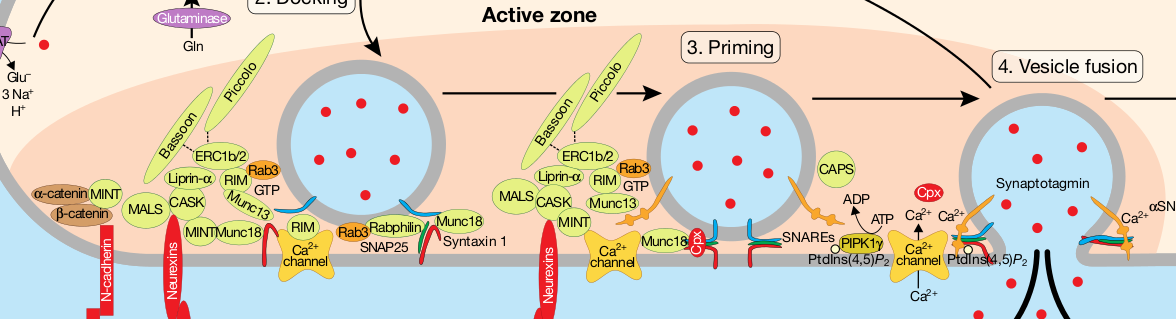
\includegraphics[width=0.6\textwidth]{actzone.png}
    \caption{An illustration of the proteins identified to be involved in the active zone network\autocite{chua_architecture_2010}.}
    \label{fig:actzone}
\end{figure}

%function of the active zone network? What does it do?

%what is community detection?
\section{Protein complexes and community detection}

As mentioned in the previous section it is possible to analyse PPI networks to detect protein complexes and functional groups.
This has recently been achieved through use of Community Detection\autocites{chen_identifying_2013,wang_recent_2010}, which uses various methods to find community structure in graphs.

%what is community structure?
Community structure is described as a characteristic of graphs which have many connections within sub-groups but few connections outside that group\autocite{newman_communities_2012}.
Unfortunately, this description is not specific on exact measures for a graph to have community structure.
Community detection algorithms are simply tested on graphs that are agreed to exhibit community structure with the aim of finding the pre-defined communities.

%describe how these algorithms usually work
There are two main approaches to the problem of Community Detection: traditional hierarchical methods and more recent optimization based methods\autocite{newman_communities_2012}.
Hierarchical methods were developed in the field of sociology and involves grading nodes by how highly connected they are in the network and then using this value to group nodes into communities.
Optimization based methods involves a different measure known as betweenness, which is analogous to the current flowing along edges if the graph were an electric circuit, and then allows a reductive technique where edges are removed iteratively to reveal sub-graphs without connections between them.

%example paper using community detection on ppi graphs?


%what is protein-protein interaction prediction?
\section{Protein-protein interaction prediction}

Protein interaction prediction was developed to solve the problem of incomplete and unreliable interaction data by combining both direct and indirect information\autocite{qi_learning_2008}.
Direct information are the result of experiments, such as yeast two-hybrid, intended to directly find protein-protein interactions.
Indirect information includes biological data that was not gathered directly to find interactions, such as gene expression data.
More information on the data sources can be found in the following section \ref{back:sources}.

%what are features?
To predict a protein interaction we need to have a value or sequence of values from which to make our guess as to the existence of an interaction.
For each interaction this set of values are known as features.
The bulk of the work in this project involved obtaining these values for every feature necessary to train the classifier and classify the interactions of the synaptic network.

%what is the classifier
The classifier is a machine learning algorithm that can learn from a labelled training set how to sort these vectors of features into the appropriate category. %citation to Murphy?
However, these algorithms cannot make predictions unless the training data is informative.
Also, the training data must be an accurate representation of the case the algorithm is planned to be applied to.

%why do we want to predict protein-protein interactions?
%reference to ENTS and similar projects aiming to make full interactomes
%how this is different to our goal
Completing the interactome of a given organism from incomplete data is a major goal for some works in the protein interaction field, such as \textcite{rodgers-melnick_predicting_2013}.
The goal in this project is to appropriately weight interactions in a PPI network to improve the performance of a Community Detection algorithm.

%what's the point in weighting connections?
Weakly interacting proteins will have a lower confidence in their interacting at all, as it will have been observed less frequently.
Therefore, by weighting the interactions in a PPI network according to our confidence we can also make the PPI network reflect more closely the true situation.

%what data sources were used to predict protein-protein interactions?
\section{Data sources and networks}
\label{back:sources}

%Different types of sources used with reference to other works
Many different data sources were considered for inclusion in this project.
The full list can be found in Appendix \ref{datasources}.
These different data sources fall into categories described in table \ref{tab:sources}.

\begin{table}
    \centering
    \begin{tabular}{l c}
        Data source type                                & Examples \\
        \hline
        \multirow{3}{*}{Primary interaction databases}  & DIP\autocite{xenarios_dip_2002} \\
                                                        & HIPPIE\autocite{schaefer_hippie:_2012} \\ 
                                                        & BioGRID\autocite{stark_biogrid:_2006} \\
        \hline
        \multirow{2}{*}{Associated features}            & Features derived from Gene Ontology\autocite{ashburner_gene_2000} \\
                                                        & Those used in \textcite{rodgers-melnick_predicting_2013} \\
        \hline
        \multirow{2}{*}{Other PPI prediction resources} & STRING\autocite{vonMering_string_2005} \\
                                                        & InterologWalk\autocite{gallone_bio::homology::interologwalk_2011} \\
    \end{tabular}
    \caption{A table summarising the different sources of data used in the course of the project.}
    \label{tab:sources}
\end{table}

%why they were chosen
The indirect sources of data were chosen based on usage in the literature, such as in the case of Gene Ontology\autocite{qi_evaluation_2006}.
Direct data sources were listed by investigating all of the available databases which could be of use and choosing from these.

\section*{Conclusion}

The goal of this project involved obtaining weights for a PPI network correlated with the strength of different protein interactions to improve the performance of a Community Detection algorithm.
Improving the performance in this way, it was hoped would produce new insight into protein interactions that could cause disease.

  \chapter{Methodology}
\label{methods}
%promises made in other sections:
% * description of disease enrichment method

%intro to the methods
Feature extraction was the predominant component in this project and involved turning the various data sources involved into usable features in a machine learning framework. 
This allowed the Classifier to be trained in a traditional way. 
%FIN: what would a non-traditional way be?  
The chosen Community Detection method, a Spectral Modularity algorithm, is also described. 
%FIN:why was it chosen? 

\section{Feature extraction}

Features are the processed form of the data we use to make predictions about a given interaction between pairs of proteins and is defined mathematically in the following text.
The process of taking a retrieving these from biological databases is referred to as feature extraction. 
%FIN: typo 
This commonly involved mapping between protein identifiers and indexing large tables automatically, but also involved many other small pieces of scripting. 
%FIN: mention non-standardisation/alternative identifiers used in different data sources -I think you need to make it clear how difficult the data collection was especially as a novice to the available databases and data formats

% going through posing the problem in terms of probability
In supervised learning problems we wish to learn a mapping between input variables and output variables given a training set.
Defining this training set rigorously, it consists of input variables $\pmb{x}$ which are typically vectors of values known as features.
The output variables in a classification problems are a set of labels\autocite[2]{murphy_machine_2012}: $y$.
In the case of binary classification these are simply either 0 or 1.
Therefore, given $N$ training vectors $\pmb{x}_{i}$ and training labels $y_{i}$ we can define our training set $\mathcal{D}$ for $N$ data points as:

\begin{align}
    \mathcal{D} = \left( ( \pmb{x}_{i}, y_{i} ) \right)_{i=1}^{N}
\end{align}

%an example?  

%pose our problem
Our problem involves taking various types of biological data, such as entries from biological databases indicating that proteins are involved in the same part of a cell and using these as features.
The training labels are either an interaction (a one) or a non-interaction (a zero).
Interactions are taken to be any interactions in the iRefIndex\autocite{razick_irefindex:_2008} database with over 50\% confidence.
%FIN: why, what is this db? consolidated database
Non-interactions are random binary combinations of Entrez protein IDs, which is a method applied in other works\autocite{qi_evaluation_2006} to create negative training examples.
%FIN: created by you how and from what dataset, hell cite the script/ipynb you used
These are also checked against the iRefIndex database to ensure they are not accidentally known interactions.
There are approximately 600 non-interactions for every true interaction.

What we would like to estimate is the posterior probability of an interaction existing given a new feature vector after training our classifier.
%FIN: typo/missing word
For any model $\mathcal{H}$ and a new feature vector $\pmb{x}^{*}$ we can express this using Bayes theorem:

\begin{align}
    p(y^{*} = 1 | \pmb{x}^{*}, \mathcal{D}, \mathcal{H}) = \frac{ p(\pmb{x}^{*}| y^{*} = 1 , \mathcal{D}, \mathcal{H}) p( y^{*} = 1 | \mathcal{D}, \mathcal{H})}{ \sum{y^{*}} p( \pmb{x}^{*} | y^{*}, \mathcal{D}, \mathcal{H})}
\end{align}

The posterior probability is $p(y^{*} = 1 | \pmb{x}^{*}, \mathcal{D}, \mathcal{H})$.
The likelihood is $p(\pmb{x}^{*}| y^{*} = 1 , \mathcal{D}, \mathcal{H})$
The prior is $p( y^{*} = 1 | \mathcal{D}, \mathcal{H})$.
The marginal likelihood is $\sum{y^{*}} p( \pmb{x}^{*} | y^{*}, \mathcal{D}, \mathcal{H})$.
Where $y^{*}$ and $\pmb{x}^{*}$ are a new label and feature vector, respectively.

We explicitly apply a prior to the probability of interaction based on the expected ratio of interactions to non-interactions stated in \autocite{qi_evaluation_2006} of $1/600$.
%FIN: what was Qi's justification for this value? Presumably observed ratios - cite the justifying paper if it wasn't Qi
This will be described in more detail in section \ref{bayes}.

\subsection{Protein identifier mapping}

Mapping from one protein identifier to another became a significant problem in this project.
%FIN: so a few of my earlier comments will be redundant to this section so reference from those sections to here 
Unfortunately, most Biological databases maintain their own indexing method to identify different genes and proteins.
New data sources being integrated into this project would often be using a different identification scheme to the NCBI Entrez GeneID originally chosen to use in the \ac{PPI} network.

%what the Entrez identifier is -  as opposed to other protein identifier schemes - cite NCBI web pages
Genes are defined by their amino acid sequence, but this is a long series of letters and the number of genes is much smaller than the possible combinations of these letters.
For the sake of posterity databases containing information about genes typically apply an identifier for each gene that is much shorter and can encode other information about the gene.
%FIN: commonly referred to as accessions 
The Entrez GeneID identifier is relatively simple, just consisting of a number generated when the gene was added to the database\autocite{maglott_entrez_2007}.

%other protein identifier schemes and mapping between them
Other popular schemes include the Ensembl identifier from the Ensembl database\autocite{hubbard_ensembl_2002}, Uniprot identifiers from the Uniprot database\autocite{consortium_universal_2008} and even those used only for specific databases such as \ac{DIP} identifiers\autocite{xenarios_dip_2002}.
Mapping between these different identifiers is difficult as each identifier may map to none or many in another database.
The reason this happens is due to isoforms of different proteins; different amino acid sequences can code for a protein with the same name.
%FIN: alternative splices of the same gene can produce different proteins, every gene is made of introns and exons, substrings which don't code for the amino acids in the protein and those that do respecitvely.  Expressed proteins are generated from any of several combinations of introns and exons (see http://en.wikipedia.org/wiki/Alternative_splicing).  Alt splicing is really important in eukaryotes and is one of the big explanations between the very low number of genes we found when we sequenced the human genome compared to the predicitions.
%FIN: the other source of 'isoforms' is when a piece of DNA is duplicated and have diverged a little in sequence between copies (older literature referred to alleles as isoforms which are slightly different as these are alternative forms of a gene such as say a gene for blue eyes or brown eyes (although that may actually be a polygenetic trait))
%FIN: you've also missed an issue with the multiple mappings of mistakes and errors, also these mistakes and errors being differentially fixed or propagated through databases.  A lot of the big source databases are public goods where many author's contribute and curation is mostly automated so have problems.  A fun and amusing example of finding accessions in databases that have been reformatted automatically by someone using excel and not noticing http://www.biomedcentral.com/1471-2105/5/80

%methods used during the project, with references to appendix notebooks
Various tools exist to map from one protein identifier to another: Ensembl's BioMart\autocite{smedley_biomart_2009} is a versatile web-based tool, for example.
In this project, simple conversion tables from NCBI's Gene\autocite{maglott_entrez_2007} ftp server were primarily used.
Another tool used was the Uniprot\autocite{consortium_universal_2008} online service web service.

% talk about the problem of canonicalisation
Unfortunately, using any of these services there will be a number of IDs which cannot be converted and many IDs mapping to the same Entrez ID as different protein isoforms are picked up.
%FIN: this isn't always the explanation - for example one database might contain say several different crystal structures done of a protein which will all theoretically map from many identifiers relating to each of these structures to one identifier of the raw sequence in genbank
One way to avoid this problem is to only refer to a single canonical form of any given protein and find this protein in other databases through its amino acid sequence.
%FIN: a benefit of this method is also that it can be used to find mis-labelled proteins: if you searched just for all data related to protein X, but someone had done a load of work on something they called protein Y but was actually protein X. If you didn't search by sequence you wouldn't find data 
This ensures that when referring to an interaction between two identifiers the interaction is always simply between two proteins.
%FIN: also note why the amino acid sequence is better than using the nucleotide sequence because it is the actual form of the protein and is derived after all the alternative splicing/isoform issues 

% how using Entrez identifiers risks becoming gene interaction prediction
% or "What Entrez isn't"
Otherwise, as in this project, the interaction is detected between two Entrez IDs; which corresponds to an interaction between genes - possibly only a single interaction between combinations of the isoforms of each gene.
%FIN: exactly, also worth putting the limitation in of not directly testing co-localisation and co-expression (i.e. temporal and spatial localisation allowing interaction)
Unfortunately, this means that this project is only concerned with gene interaction prediction until the Entrez IDs have been carefully canonicalized.
This is not really a problem, as we are only aiming to provide a weighting to a graph, rather than provide an accurate prediction of interaction between proteins.
%FIN: to be less negative maybe say you will still identify possible interactions but may not identify all of them (as you are only checking one isoform etc).  This can still be informative if it is a new predicition which is later validated

% how iRefIndex solves this problem and should have been used from the start
% with reference to storing the sequences of each protein involved to maintain unambiguity
A solution to this problem is provided by the iRefIndex\autocite{razick_irefindex:_2008} database, which combines many databases and stores canonicalized entries.
Using this database, it would be possible to ensure that the proteins used in a future project would be reliable canonical proteins.
Additionally, each protein of interest should ideally be stored with reference to its sequence in, for example, FASTA format.
%FIN: be explicit amino acid sequence rather than protein sequence

%description of feature extraction code
\subsection{Dedicated code: ocbio.extract}

% link to the notebook on using this code
% but update it to explain what custom generator options are
To keep track of the various different data sources and assemble the features into vectors to be used in the classifiers a dedicated piece of code was required.
The code developed is written as a python module called ocbio.extract.
Usage and development notes for this program are referenced in Appendix \ref{app:ocbio}.

\subsection{Gold standard datasets}
%material on the problems with choosing between gold-standard datasets
% with reference here to the section in Qi's thesis


%original work on \ac{DIP} (justified choice from previous work)
The database of interacting proteins (\ac{DIP}) is a database of interactions proven by small-scale experiments\autocite{xenarios_dip_2002}.
Each interaction added is hand curated so it was expected as a reliable training set.
Also, this database was used as a training set in \textcite{qi_evaluation_2006}.

%problems with \ac{DIP}
%why \ac{HI\ac{PPI}E} is better suited
Unfortunately, problems were found with \ac{DIP} as a training set. 
%FIN: I don't understand - explain what these problems are/were
Features derived from interaction databases would win out in importance versus all indirect features as shown in figure \ref{fig:unbalanced}.
\ac{HI\ac{PPI}E} was also tested as a training set, but this lead to the same problem.
%FIN: so which did you use?

%example feature importance graph
\begin{figure}
    \centering
    \setlength\figureheight{3in}
    \setlength\figurewidth{4in}
    \InputIfFileExists{\imagedir/unbalanced.weighting.tikz}{}{\textbf{!! Missing graphics !!}}
    \caption{An example of an unbalanced set of feature importances plotted after fitting a Random Forest classifier to a dataset containing interaction database derived features. Feature indexes are not as described in table \ref{tab:fvectors}.}
    \label{fig:unbalanced}
\end{figure}

%After removing interaction databases 
It was decided that only indirect features should be used in the trained supervised classifier and direct evidence integrated into the final weightings in an explicit Bayesian method described in section \ref{bayes}; the results of which are described in section \ref{bayesresults}.
Once these databases were removed the performance of the classifier was drastically lower.
However, all of the available features had more closely distributed importances in the final classifier, as shown in section \ref{importances}.
%FIN: this isn't obvious to me - you need to explain why balance set of features is important 


%iRefIndex as a final solution?
To train the final classifier the iRefIndex\autocite{razick_irefindex:_2008} database was used to find positive interactions due to its effective protein identifier mapping ability, as described above.
Again, non-interactions were generated as random combinations of Entrez Gene IDs.
These were also checked against the positive interactions to ensure known interactions were not present.

\subsection{\ac{PPI} prediction features}

%planned features, describe the list of possible features which was created
%put it in the appendix as a table, or otherwise somehow
\ac{PPI} prediction features are a set of values for each interaction considered, if it is a real or non-interaction.
This arrangement is illustrated in figure \ref{fig:fvectors}.
The features used are described by index in table \ref{tab:fvectors}.

%this could be a good place to put that diagram of exactly what a feature vector is
\begin{figure}
    \centering
    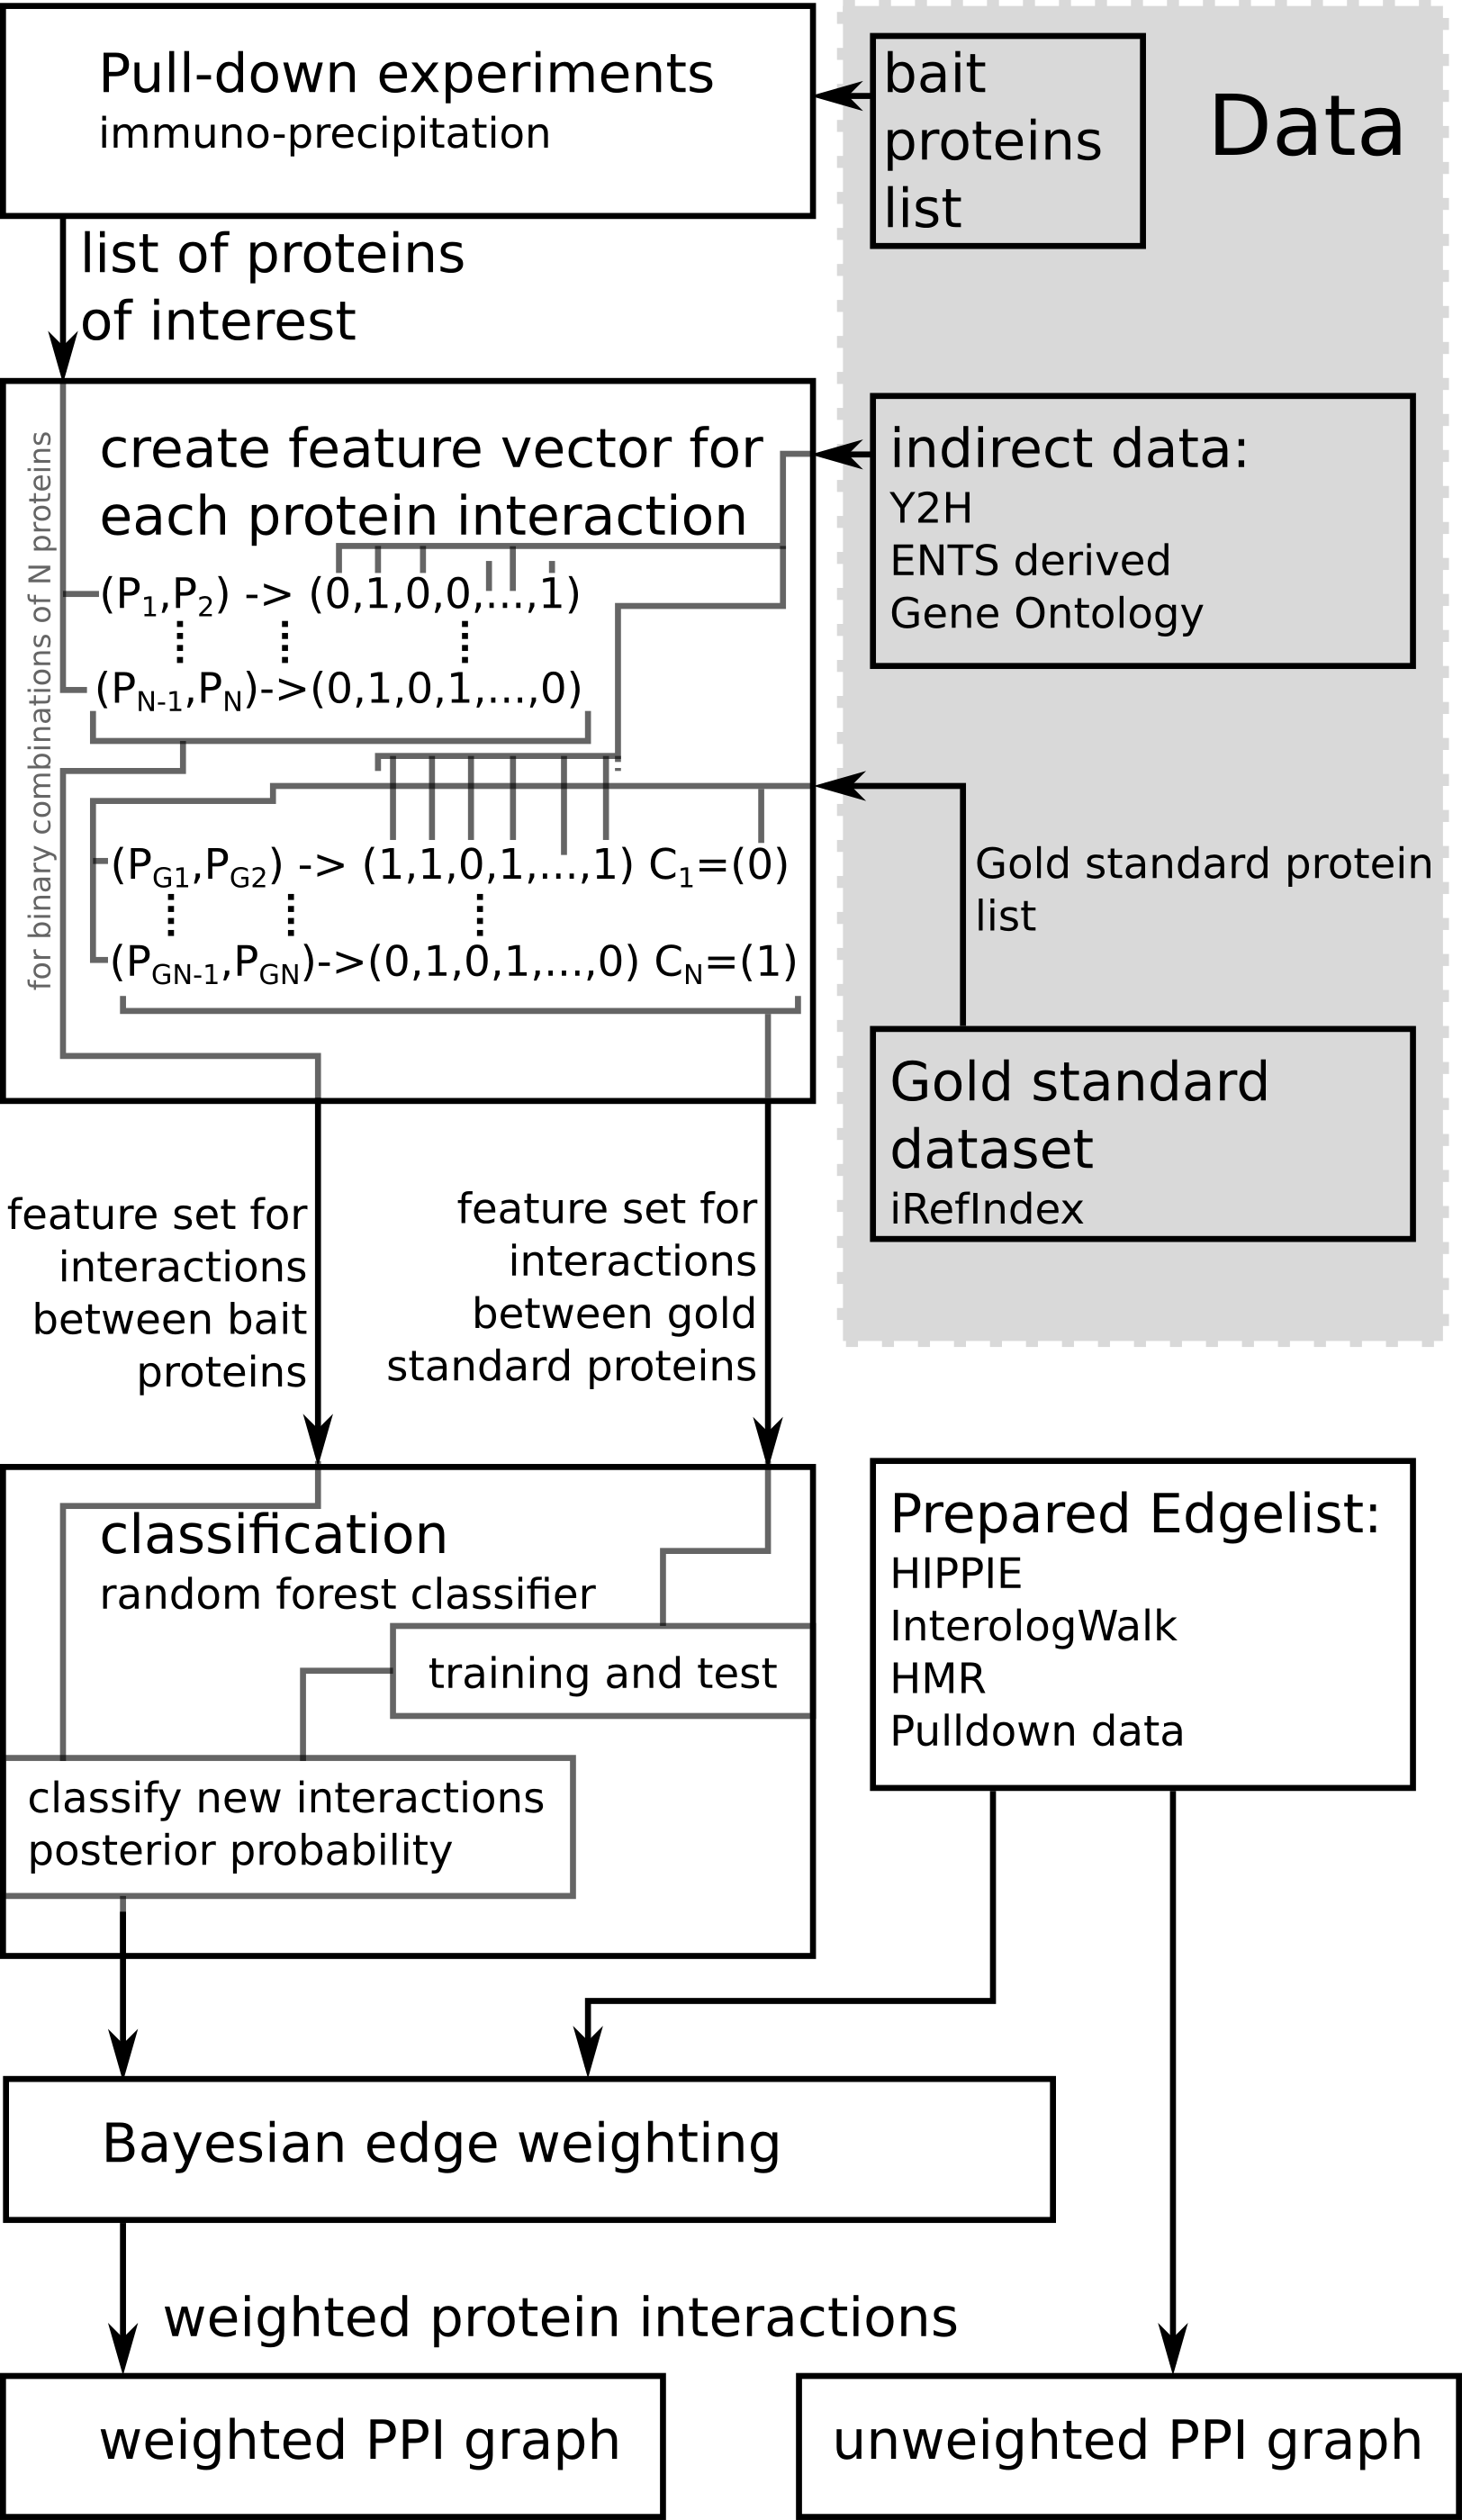
\includegraphics[width=0.8\textwidth]{fvectors.png}
    \caption{A diagram showing the structure of feature vectors and their relationship to the project as a whole. This figure is based on a similar flow chart shown in the project proposal.}
    \label{fig:fvectors}
\end{figure}

\begin{table}
    \centering
    \begin{tabular}{l c p{0.5\textwidth}}
        Feature         & Indices & Description \\
        \hline
        Gene Ontology   & 1-90    & Described in section \ref{go}, with individual indices described in Appendix \ref{app:go}. \\
        Y2H             & 91      & Y2H experimentally derived feature \\
        ENTS derived    & 92-198  & Features used by the ENTS classifier, described by index in supplementary table for \textcite{rodgers-melnick_predicting_2013}. \\
        ENTS summary    & 199     & Prediction result of the classifier in \textcite{rodgers-melnick_predicting_2013}. \\
    \end{tabular}
    \caption{Each feature used in the final classifier is described by index.}
    \label{tab:fvectors}
\end{table}

%details of what classifiers were chosen and about scikit-learning
\section{Weighting Protein Interactions}

%classification as a weighting tool
The classification problem we are solving is different in that we are really trying to obtain a realistic weighting of interactions for use in a \ac{PPI} network.
%FIN: different from what? 
Classification is normally concerned about picking a decision threshold to classify examples into categories.
However, in this case the output of our process is the posterior probability of the model given a new example.

%introduce scikit-learn
To produce this output the chosen tool was the Python package Scikit-learn\autocite{pedregosa_scikit-learn:_2011}.
Each classifier implemented in this package has a similar interface allowing modular code to be written.
In addition, this package is actively developed with all the required classifiers having efficient implementations.
%FIN: also one of most widely used packages 
% explain why we tried the algorithms that we tried
The following sections describe the three classifiers chosen.
These were a logistic regression model, a random forest model and a support vector machine.
Each of these involved tuning a number of hyper-parameters.

\subsubsection*{Hyper-parameters}
%describe the different parameters varied in scikit-learn by name
%FIN: explain what a hyper-parameter actually is  
Each of the Classifiers used has hyper-parameters which will affect its performance.
These hyper-parameters are described in table \ref{tab:hyper} for each of the models used in the project.
The optimal values for these found can be found in section \ref{gridresults}, table \ref{tab:gridresults}.

%table of the different hyper-parameters
\begin{table}
    \centering
    \small
    \begin{tabular}{p{0.2\textwidth} c p{0.5\textwidth}}
        
        Classifier                                  & Hyper-parameters     & Description \\
        \hline
        Logistic Regression                         & C                         &  Inverse of regularisation strength, the $\alpha$ parameter in section \ref{logreg}. \\
        \hline 
        \multirow{3}{*}{\parbox{0.2\textwidth}{Support Vector Machine}}     & kernel                    &  The kernel used. Three options: linear, \ac{RBF} and polynomial. \\
                                                    & Gamma($\gamma$)           &  Kernel coefficient. \\
                                                    & C                         &  As with Logistic Regression, a penalty parameter. \\
        \hline 
        \multirow{2}{*}{\parbox{0.2\textwidth}{Random Forest}}              & N estimators              &  Number of trees used in the forest. \\
                                                    & Max features              &  Number of features considered when looking for splits, part of the problem of finding the best decision at each node described in section \ref{randomforest}. \\
        \hline 
        \multirow{2}{*}{\parbox{0.2\textwidth}{Extremely Randomized Trees}} & N estimators              &  As with Random Forest. \\
                                                    & Max features              &  As with Random Forest. \\
    \end{tabular}
    \caption{Summary of the hyper-parameters described in the Scikit-learn \autocite{pedregosa_scikit-learn:_2011} documentation to be tuned for each of the models considered.}
    \label{tab:hyper}
\end{table}


\subsubsection*{Logistic Regression}
\label{logreg}

%with reference to Murphy
Logistic regression is a linear model being used for classification.
%FIN:binary classification  
It is equivalent to a linear regression model transformed through a sigmoid function\autocite[376]{murphy_machine_2012}, denoted here by $\sigma$:

\begin{align}
    p(c=1|\pmb{x}) = \sigma(b + \pmb{x}^{T}*\pmb{w})
    \label{sigmoidtransform}
\end{align}

In equation \ref{sigmoidtransform} $\pmb{x}$ is the vector of features and $c$ is the class label - in our case $1$ is a real interaction, $0$ is a non-interaction.
The weights and biases are the parameters of this model, expressed in the above equation as $b$ and $\pmb{w}$, respectively.

This divides the points in the dataset by a hyperplane, classifying the points on each side into different classes.
For data that is linearly separable, this produces a classifier that will make no mistakes on the test data.
Unfortunately, the data we are working with is not linearly separable as shown in section \ref{dataviz}.

%How is it trained?
To find the parameters the log likelihood of this model must be maximised; corresponding to the maximum likelihood solution.
The log likelihood for this model, for N feature vectors, is:

\begin{align}
    L(\pmb{w},b) = \sum_{n=1}^{N} c^{n} \log \sigma(b + \pmb{w}^{T}\pmb{x}^{n}) + (1 - c^{n})\log (1 - \sigma(b + \pmb{w}^{T}\pmb{x}^{n}))
\end{align}

%describe what the C parameter is
Regularisation of the weights represents a prior belief that the weights should not increase without bound.
In a case where the data is linearly separable and where regularisation is not applied the weights will increase without bound to produce extremely confident classifications\autocite[381]{barber_bayesian_2013}.
To stop this from happening we apply a penalty term, $\alpha$, to the size of the weights:

\begin{align}
    L'(\pmb{w},b) = L(\pmb{w},b) - \alpha \pmb{w}^{T}\pmb{w}
\end{align}

Tuning this hyper-parameter is the goal of a grid search when training a Logistic Regression model.
%FIN: explain grid-search 
\subsubsection*{Support Vector Machines}
%FIN: you are a big fan of Murphy 
%with reference to Murphy
Logistic regression can be generalised to apply kernel functions to the input features to obtain better classifications.
Support Vector Machines exploit this while also applying a different objective function intended to avoid overfitting\autocite[383]{murphy_machine_2012}.
The objective in placing the hyperplane for a Support Vector Machine is a "maximum margin" in that is attempts to maintain the same distance from the closest opposing class points.
%FIN: typo/missing word

%success of these models?
These are often successful classifiers in practice.
Applications include text categorisation, hand-written character recognition, image classification and biosequences analysis\autocite{cristianini_introduction_2000}.

%describe the hyper-parameters?
The hyper-parameters for a Support Vector Machine control the kernels, along with the regularisation parameter as described for logistic regression in section \ref{logreg}.
%FIN: explain what a kernel is and how \ac{SVM}s can classify non-linearly seperable unlink logit by transformation to feature space
Two hyper-parameters which can be tuned during a grid search operation are the degree of polynomial kernels if chosen and the gamma coefficient of the kernels.


\subsubsection*{Random Forest}
\label{randomforest}

Random forests operate as a combination of many decision trees.
Decision trees are intuitively simple in that it consists of a series of comparisons arranged in a tree as shown in figure \ref{fig:dectree}.

\begin{figure}
    \centering
    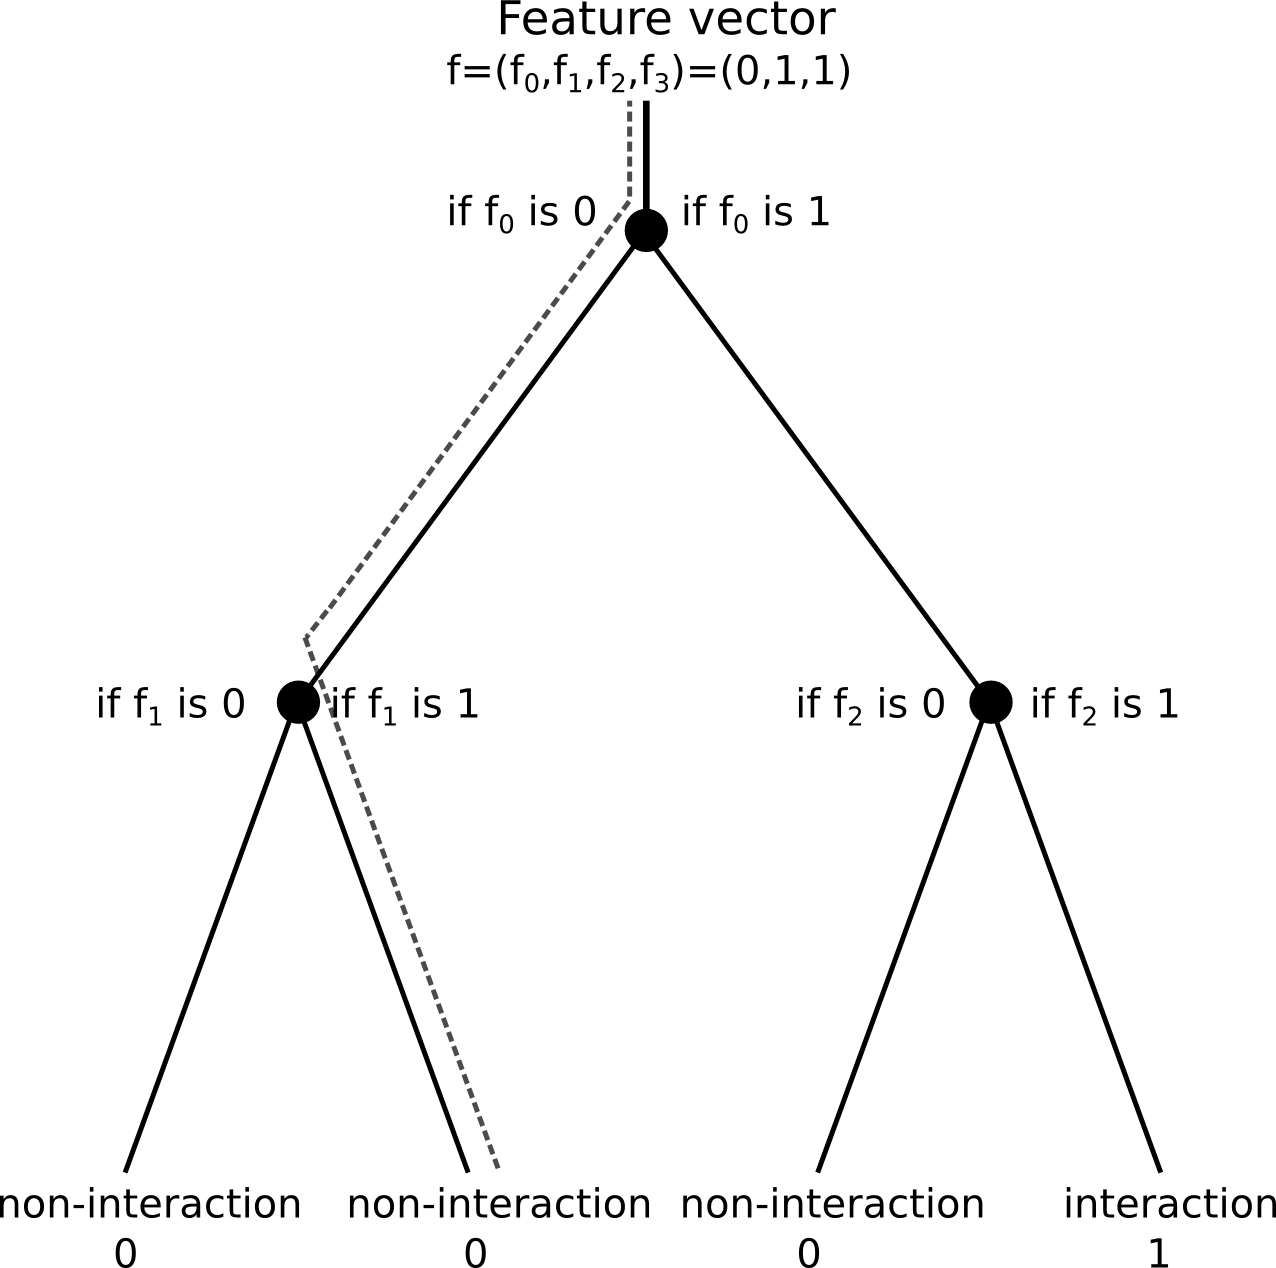
\includegraphics[width=0.8\textwidth]{decisiontree.png}
    \caption{A simple example decision tree, illustrating the process of sequential, dependent decisions. Based on an image obtained through Wikimedia\autocite{wkmdacommons}.}
    \label{fig:dectree}
\end{figure}

In this way decision trees are both simple and tractable methods for using a feature vector to classify inputs and there are many automated ways to generate effective decision trees.
The problem in the design of a decision tree is which comparison to choose at each node, described as how to partition the data\autocite[544]{murphy_machine_2012}. %redundant citation here?
There are several implementations of algorithms to achieve this and a full description can be found in \textcite[544]{murphy_machine_2012}.
Other advantages of decision trees include the ability to handle a mixture of discrete and continuous inputs, automatic variable selection, scaling to large datasets readily and the ability to handle missing inputs, with modification.
%other strengths of decision trees?

%describe split function? probably not worth going into this.

%then explain the problems with decision trees, variance etc
Unfortunately, despite the strengths of decision trees there are still problems with stability: small changes in the input data can produce large changes in the output\autocite[550]{murphy_machine_2012}.
The random forest algorithm addresses this problem by providing redundancy; multiple trees are grown and their results averaged.
%FIN: how many trees?
For M trees trained on different subsets of the data\autocite[551]{murphy_machine_2012}:

\begin{align}
    f(x) = \sum_{m=1}^{M} \frac{1}{M} f_{m}(x)
\end{align}

Where $f_{m}(x)$ is $m$th tree. This is simply averaging the results of the trees and is known as bagging.

%with reference to Qi and ENTS, showing good performance on this problem
With the ability to work on large datasets and mixing continuous and discrete data these types of classifiers would appear to already be well suited to this problem.
%FIN: maybe say well theoretically suited and then show in reality with the citations 
This is what has been observed in the literature, with these classifiers achieving the best performance despite different types of biological data being used\autocites{qi_evaluation_2006,rodgers-melnick_predicting_2013}.
Due to these reports in the literature it appeared that this classifier would be the best choice for our protein interaction prediction task.

%expand on how much better they were etc? in different places?

\subsubsection*{Other options}

% what other algorithms could we have tried but didn't
Other options considered for our classification problem, but not included in the project due to time constraints included Feedforward neural networks, Naive Bayes and Beta regression.
Naive Bayes in particular would have required modifying the code from Scikit-learn to deal with data from multiple different distributions or implementing Weka's solution of kernel density estimated distributions for each different feature\autocite{john_estimating_1995}.
%FIN: explain why 
Beta regression would have been very suitable for the task and is suggested as future work, described in the following section.

\subsubsection*{Beta regression}

%what is beta regression? quickly
Beta regression is a generalised linear model is one in which the output variable is distributed according to a Beta distribution\autocite{smithson_better_2006}.
%FIN: typo/missing word
A maximum-likelihood solution to this model can be found and the resulting model fit in the same way as a standard regression model.
%FIN: typo/missing word

%why this would also have been a good idea, if we didn't have to implement it ourselves
True protein interactions are not something which can be assumed in a protein interaction prediction task.
Many proteins are known to be very likely, but others are less confidently classified, as reflected in the \ac{HI\ac{PPI}E} database's confidence scoring system\autocite{schaefer_hippie:_2012}.
%FIN: typo/missing word

To train a classifier a training set of true and false interactions is required and this cannot be supplied without thresholding the database at an arbitrary confidence value.

Beta regression avoids this problem as it allows the confidence values to remain a part of the regression process.
Using this we can build a model and update our belief on the likelihood of interaction in a Bayesian framework much more easily.

%FIN: actually this is pretty cool, note to self read up on Beta regression 
\subsection{Classifier testing}
\label{classifierverification}

%Tests we planned to use on each classifier:
%  mention cross-validation
%  learning curves
%  simple accuracy value
%  grid search
%  \ac{ROC}
%  Precision recall
%  test interactions
%  

% consider using paragraph headings in this section
Various measures were applied to each classifier to estimate their performance in different ways.
These tests included simple accuracy measures applied over learning curve and grid searches along with plotting \ac{ROC} and precision-recall curves.
Grid searches of parameter values were used to find optimal hyper-parameters.

% was or will be?
Cross-validation was applied to tests during parameters searches and when plotting learning curves to get a statistical estimate of the reliability of the metrics applied to the classifier\autocite[152]{witten_data_2011}.
%FIN: you don't really explain what CV and why you can't just optimise the models performance directly on the test set
As the training set is relatively large, these were applied as random sub-samples of the full data set, but stratified to maintain the same proportion of zeros to ones as in the full training set.
This is important as it must reflect the expected ratio for real protein interactions to non-interactions.

\subsubsection*{Pipeline}

%what is a pipeline? why did I use one?
A pipeline is a combination of algorithms intended to run on the data in sequence after the data has been split into training and test.
In the case of this project the pipeline involved three components: a mean value filling imputer, a standard scaler and the classifier itself.
The imputer simply replaced missing values in the training data with the corresponding mean value for that column.
Scikit-learn's standard scaler centers the data at zero mean and unit variance.

%FIN: need to explain/just why you need to normalise data and gracefully handle missing data

\subsubsection*{Learning Curves}
% learning curves, what are they? and why?
Learning curves, as in the notebook referenced in Appendix \ref{app:classtrain}, were used in this project to ensure that the number of samples used in a grid search was sufficient.
The learning curve plots the accuracy of a classifier after it has been trained using cross-validation on a varying number of samples.
%FIN: most importantly they can diagnose common classifier issues (bias/variance) 
%example learning curve?
%still pending, worth it if page count allows

\subsubsection*{Grid search}
% grid search
A grid search is a cross-validated test measuring accuracy testing the classifier with a variety of different hyper-parameters.
Classifiers, such as a Logistic Regression model, have some number of hyper-parameters.
A Logistic Regression model, for example, has a single hyper-parameter so that the grid search for this model simply involves varying this parameter to obtain the optimum performance on the test set.
%FIN:repeat hyper-parameter identity in logististc regression - regularisation

\subsubsection*{Accuracy}
% accuracy value
The accuracy value plotted in the learning curve and used in grid searches of parameters values is simply the proportional of correctly classified instances in a training or validation set.
Typically, the protein interaction prediction problem is sparse, in that there are very few interactions for the large number of non-interactions.
This is reflected in the accuracy in that a classifier that simply always predicts zero can still achieve a very high accuracy.
Using this accuracy value is therefore problematic and this requires the other measures employed, such as \ac{ROC} and precision-recall \ac{AUC} values.

\subsubsection*{\ac{ROC} curve}
% explain what those are
A Receiver Operating Characteristic, or \ac{ROC}, curve plots the variation in true positive to false positive rate as the threshold of classification is varied.
This makes it useful as an illustration of the tradeoff possible with this particular classifier.
The Area Under Curve, or \ac{AUC}, value is the area under this line.
A higher \ac{AUC} value corresponds to a better classifier, although there is some controversy surrounding this\autocite{hanczar_small-sample_2010}.
These concerns center on the problems of small sample sizes, which are not the case in this project.
%FIN: maybe add in a wee truth table of TP, TF, FP, FF 
\subsubsection*{Precision-recall curve}
%precision recall
A precision-recall curve plots the precision of a classifier against its recall as the threshold of classification is varied.
The precision is defined as the number of true positive results over the number of total positive results.
Recall is defined as the number of true positive results against the number of available positive examples
The area under the curve is used to gauge the classifier's effectiveness.
%FIN: may as well add the equations in for precision and recall, TP, TF, FP, FF - I mean you did put down baye's rule earlier 
%example \ac{ROC} curve?
%example precision recall curve?

\subsection{Missing data}
%how was missing data dealt with?
Before classification could be performed the missing data in the feature vectors had to be imputed.
This was performed by filling the missing values with the mean value of that feature.
This is a common technique that is applied if it is likely the data is missing at random.
In this case the data that is missing is due to mismatches in protein identifier mapping dictionaries, which is likely random and independent of the interaction prediction task.
%FIN: link back to imputer discussed earlier, if you are having a section on this you could add a section on data normalization

\subsection{Bayesian weighting}
\label{bayes}
%description of the method used to weight interactions after the classifier was found to be insufficient

%justification for using this method, the problem with supervised classification?
%CHECK THIS ISN'T FOUND ELSEWHERE ALREADY
Weighting interactions using the posterior distribution of a probabilistic model requires that the model accurately represents beliefs about the system being modelled.
Supervised classification requires that true interactions are known in order to find the parameters of the model.
Unfortunately, in this problem we cannot know for certain whether an interaction is real or false.
Therefore, when fitting a supervised model we only obtain, at best, an accurate predictor for the interaction database used to fit the model.

%the prior on the edgelist
As the \ac{PPI} network edges we plan to weight have already been defined through combining different interaction databases we already have a strong prior on the existence of these interactions.

Using the classifier on its own can then, at best, reproduce one of the databases used to create this network and many of the interactions will be incorrectly weighted much lower than expected.
The solution is to treat both the result of the classifier and the edgelist inclusion as observable events dependent on the latent ``interaction'' variable.
Along with these variables, we can also include other protein interaction prediction resources, such as \ac{STRING}\autocite{von_mering_string:_2005}.

%naive bayes model, advantages, disadvantages
The model we have chosen to update our prior belief using assumes conditional independence of the observable variables given the hidden interaction variable.
This equates to a Naive Bayes model with a belief network as shown in figure \ref{fig:naive}.
An advantage of this model is the simplicity of its analysis.
The disadvantage is that our variables could be dependent, as the classifier is trained on some of the same interaction databases that the \ac{HI\ac{PPI}E} database is composed of.
%FIN: typo/missing word

%belief network for naive bayes
\begin{figure}
    \centering
    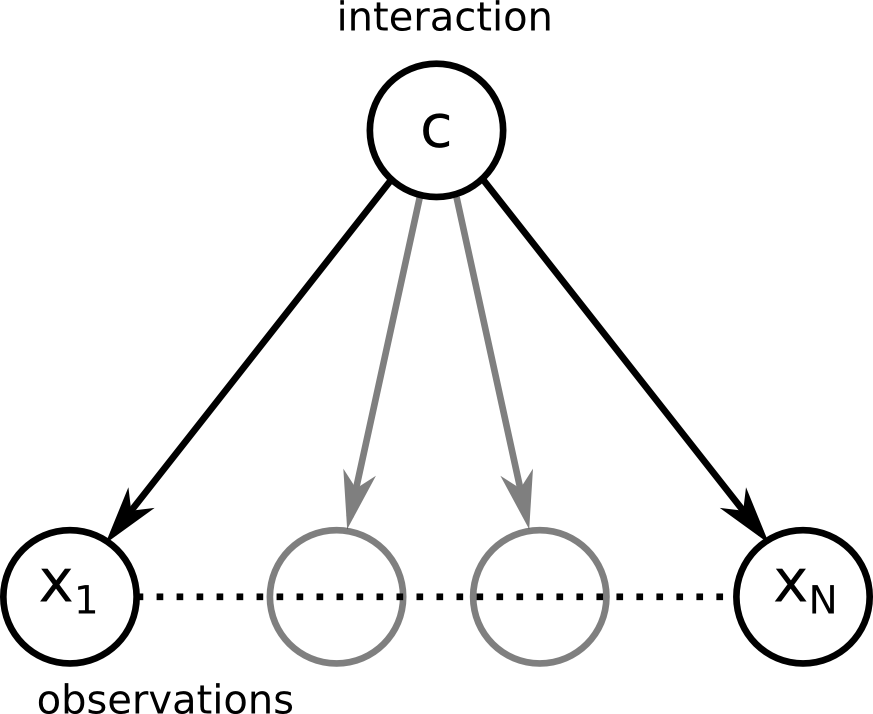
\includegraphics[width=0.6\textwidth]{naive.png}
    \caption{A belief network illustrating the Naive Bayes model, equivalent to that used for inference when weighting the interactions of the \ac{PPI} network.}
    \label{fig:naive}
\end{figure}

%updating on evidence? equations

%the importance of conservative estimates
The class label, interaction, is not observed in this model so we cannot solve to find the parameters.
%FIN: \ac{PPI} or not
To define the model, the only way to proceed is to manually define them by conservatively estimating the conditional true positive and false positive rates of the Bernoulli distributions.
Continuous distributions, such as the classifier predictions or prediction databases, must be estimated using \ac{KDE}. 
%FIN: explain \ac{KDE} acronym 

%kernel density estimation, justification from Weka
Using \ac{KDE} in conjunction with Naive Bayes is the approach used by Weka to deal with arbitrary conditional distributions\autocite{john_estimating_1995}.
%FIN: you need to explain what Weka is 
Unfortunately, this distribution is estimated using samples labeled using the protein interaction databases, so we cannot be fully confident in its predictions.
As before, a conservative estimate of its accuracy is applied through increasing the smoothing bandwidth.

\section{Measures applied to weighted and unweighted \ac{PPI} networks}

%why do we want to try weighted networks? and intro
It is hoped that a weighted graph will provide new insight into the interactions of proteins in the active zone.
%FIN: I think at this stage you need a refresher to the reader on what active zone you are talking about
For this reason, comparing the unweighted and weighted cases of the graph produced is a major goal of this project.
The following sections describe this process and the measures applied to both graphs.

\subsection{Community detection}
%FIN: section needs expansion in the areas you have noted 
%description of each of the algorithms available
%three:
%  Geodesic edge Betweenness
%  Random edge Betweenness
%  Spectral Betweenness
Three algorithms were identified for use in this project for community detection, the first two are described in \textcite{newman_finding_2004}.
Geodesic edge betweenness and random edge betweenness are based on betweenness measures to partition the graph, making them optimisation approaches.
The third, spectral modularity, was the chosen algorithm in this project.

%with reference to Colin's paper, why this is a good choice
The original advantages of spectral modularity techniques were better results in less time than competing methods in \textcite{newman_modularity_2006}.
In a recent paper, this method was compared favourably to other methods in terms of CPU time\autocite{mcleanunpub}.
Although it detected fewer communities, it maintained a higher modularity score.

%community detection code, what it does, which algorithm was used
%pending use - will see if I have time to use more than one

\subsection{Normalised Mutual Information}

%NMI theory, what is a measure of
Mutual information intuitively is the reduction in uncertainty about one random variable by observing another
Defined in terms of entropy it is\autocite{mackay_information_2003}:

%could move that citation next to the equation?
\begin{align}
    I(X;Y) = H(X) - H(X|Y)
\end{align}

Where $H(X)$ is the entropy of the random variable $X$ and $H(X|Y)$ is the conditional entropy of $X$ given $Y$.

In the case of the function we are using to perform this from Scikit-learn the mutual information is normalised by $\sqrt{H(X)\times H(Y)}$\autocite{pedregosa_scikit-learn:_2011}.
This produces a value between zero and one which reflects the redundancy of the distributions - 1.0 being exactly the same and 0.0 being independent.

\subsection{Disease Enrichment}

%Primer on what this test actually does
By linking the proteins in a cluster to known disease annotations it is possible to estimate the likelihood that a given community is involved in a particular disease.
The code being used produces a p-value to indicate this likelihood.
%FIN: explain a p-val? 

In the case of this project, due to the aims of the SYNSYS project and for simplicity, only two diseases were investigated: Schizophrenia and Alzheimer's.

%interaction between significance level and p-value


\section*{Conclusion}

This project involved a large number of varied techniques and algorithms being used on large data sets.
Many problems had to be solved in order to piece together the full project.
As each of these steps were sequential, the results section describes the results as they were gathered, in the same structure as seen above.

  \chapter{Results}
\label{results}

%intro to the results

%iterations of results - DIP, HIPPIE, Bayesian updating and reasoning behind it
% can then refer to this throughout this section.
As the project progressed the intended approach was found to be flawed and some changes were made.
The first of these was the change from a DIP-based training set to HIPPIE-based training set.
After the classification had been performed the use of a supervised classifier with this training set was found to be a poor method by itself for weighting interactions.
Using all of the data available it was possible to run a simple Bayesian alternative to continue with the weighting for the Community detection algorithm.

%Feature extraction results
\section{PPI feature vectors}

%The features extracted were X,Y,Z and the appendices explaining how this was done are A,B,C.
Many features were identified for extraction and these are described in Appendix \ref{datasources}.
Of these, only a small subset were succesfully processed into a usable form.
These are listed below and more information about each can be found in Appendix \ref{datasources}:

%more citations below?
\begin{itemize}
    \item HIPPIE database
    \item Pulldown derived features: affinity and abundance
    \item Gene Ontology, also described in section \ref{go}
    \item Yeast Two-Hybrid, also described in section \ref{y2h}
    \item ENTS derived features, also described in section \ref{ents}
    \item iRefIndex database
    \item STRING database
    \item HMR database 
    \item InterologWalk results
\end{itemize}

Of these, a smaller proportion were used in the final classifier, which neglected features directly derived from interaction databases.
The features used to train the final classifier are shown in table \ref{tab:features}.
A brief description of these features is given below.

%feature table, with information about each (size of features, categorical/ordinal/numerical, coverage)
\begin{table}
    \centering
    %tabular goes here
    \begin{tabular}{l c c c c}
        Feature         &   Size &  Type                &  Coverage on training set &  Coverage on active zone network \\
        \hline
        Gene Ontology    &  90   &  Binary categorical  &  100.0\%                  & 100.0\%                          \\
        Yeast two-hybrid &  1    &  Numerical           &  100.0\%                  & 100.0\%                          \\
        ENTS derived     &  107  &  Numerical           &  38.39\%                  & 42.74\%                          \\
    \end{tabular}
    \caption{A table summarising the components of the feature vectors used in the final classifier.}
    \label{tab:features}
\end{table}

%these subsections may be too small
\subsection{Gene Ontology}
\label{go}

%Larger features
%Gene ontology was built as a feature in the same manner as that of qi_evaluation_2006 but, without knowing their approach, we had to develop our own method of creating usable features.
The Gene Ontology\autocite{ashburner_gene_2000} is a resource of annotations for genes to indicate various characteristics in a hierarchical manner, such as cellular localisation or function.
This resource has been used in past papers\autocite{qi_evaluation_2006} and in databases such as STRING\autocite{von-mering_string:_2005} to predict protein interactions.
Intuitively, it can be used to detect when, for example, two proteins are localised in the same area of the cell - as this would increase the probability that these two proteins interact.
Details on exactly how this feature was generated can be found in the notebook reference in Appendix \ref{app:go}.

\subsection{Features derived from ENTS}
\label{ents}
%ENTS features were retreived through analysis and modification of the code published on the ENTS website, but did not have full coverage on any dataset.

These features were obtained through analysis and modification of the bundled code and data downloaded from the website of \textcite{rodgers-melnick_predicting_2013}.
In turn, most of these features were generated through the Multiloc2 program of \textcite{blum_multiloc2:_2009}.
The remaining features are pairwise combinations of conserved protein domains, which are conserved "modules" of proteins described in \textcite{janin_domains_1985}.

\subsection{Yeast Two-Hybrid results}
\label{y2h}

%description of Y2H feature
%pending

\subsection{Removed features}

%Before their removal the features that best predicted the chosen gold standard dataset were reliably those directly derived from interaction databases.
As listed above there were originally many features used in the supervised classification that were derived from interaction databases.
These were very effective in predicting interactions on the training set, as expected, but their importance in the task outweighed any other features, as shown in figure \ref{fig:unbalanced}.
It was decided that indirect features should be used in the trained supervised classifier and direct evidence integrated into the final weightings in an explicit Bayesian method described in section \ref{bayes}; the results of which are described in section \ref{bayesresults}.

%example feature importance graph
\begin{figure}
    \centering
    \includegraphics[width=0.8\textwidth]{unbalanced.weighting.png}
    \caption{An example of an unbalanced set of feature importances plotted after fitting a Random Forest classifier to a dataset containing interaction database derived features.}
    \label{fig:unbalanced}
\end{figure}

%After removing interaction databases 
Once these databases were removed the performance of the classifier was drastically lower.
However, all of the available features had more closely distributed importances in the final classifier, as shown in section \ref{importances}.
The classifier was then integrated 

%graph of feature importance from RF classifier? probably not required, will be found below.

%tables with explanation - table above now, not required.

\subsection{Data visualisation}

%describe the problem of using in proportion and out of proportion methods
For all graphs, two cases were investigated: in proportion and out of proportion.
In proportion refers to the case where the proportion of interactions to non-interactions is correct; specifically, 1 interaction to 600 non-interactions.
Out of proportion maintains the same number of interactions to non-interactions.
This is important as it is often easier to separated the data when the classes are equally split.

\subsubsection{Reducing dimensionality}
%PCA is a relatively simply and fast way to reduce the high dimensionality of our feature vector into a form that can be easily plotted.
Two methods were tested to reduce the dimensionality of the data to two dimensions so that it could be easily plotted.
The first of these is PCA, which is relatively simple with a fast implementation, and the second is t-SNE, which is more complicated but has achieved better performance in recent works.
Both of these methods are described below in more detail.

%PCA description, referencing Barber

%tSNE is more complicated, but was recommended due to reportedly good performance


%Both methods show that this data is likely to be difficult to accurately categorize as the points are not separated in a 2d space

\subsection{High dimensional plots}

%Very few graphs are able to integrate large numbers of dimensions in a meaningful way; parallel line graphs and Andrew's curves are the two we have applied.

%Explain how Andrew's curves work, what they mean.




\section{Classification of weighted PPI networks}

\subsection{Missing data}
%how was missing data dealt with?

%Justification for mean value filling.

%Accuracy as a simple measure of the performance of a classifier is difficult to interpret in the case of a heavily unbalanced classifier such as this.
\subsection{Classifier accuracy and best parameters}

%Using grid searches over the following parameter ranges we were able to search for the optimal parameters for each of the classifiers tested.

%table of the best parameters obtained for each classifier.

\subsection{ROC curves}

%An ROC curve plots the tradeoff between true positive and false positive rates, in the case of an unbalanced classifier large sample sizes are required to obtain a smooth, stable curve.

%ROC curves for the different classifiers

%differences between the classifiers and reasons for this.

\subsection{Precision-recall curves}

%what a precision recall plot is?

%precision recall curves for the different classifiers


\subsection{Feature importances}
\label{importances}

%Comparing logistic regression to random forests

%tests characterising and comparing different classifiers, results

%Treating interactions as an unobserved random variable, we were able to build a simple probabilistic model to make up for the failings of the classifier and continue with the Community Detection.

\subsection{Bayesian weighting of interactions}
\label{bayesresults}

%description of the Bayesian method of interaction weighting, with reference to the notebook on this

\section{Comparison of weighted and unweighted PPI networks}

%Here are the communities we detected in each case

%images of both sets of communities, nicely rendered

%Investigate some of the communities by eye, look at distribution of baits etc

\subsection{Graph comparison}

%comparison of using weighted and unweighted
%NMI and disease enrichment

\section*{Conclusion}



  \chapter{Conclusions}
\label{conclusion}

This project involved an array of different tools and data.
Despite many difficulties and mistakes during the planning of the project, all of the aims of the project as stated in the proposal have been met.
Despite lacking conclusive results this work represents a step towards a system for unifying diverse interaction data sources.
%However, the results obtained are not conclusive or useful.
%FIN: try and spin the positives a bit harder - what can be done to make them useful, 'this work represents a step towards that'

%project ran out time towards the end

\section{Deliverables}
%what was achieved (as a reminder)
During the course of the project a large number of data sources were tested and extracted into a machine learning workflow.
These formed large feature vector files which could be used for classification.
Three different classifiers were then trained on this data and compared.
Of these, the best was used to provide predictions to weight edges.
A Bayesian method was used to combine this with other data sources and prior knowledge to generate the edge weights.
These edge weights were then used to create a weighted \ac{PPI} graph which was then compared to its unweighted counterpart.

%problems with results
%FIN: could maybe put in what features you identified as being important as a possible source of future work


%\section{}

\section{Future work}
%repeat Bayesian approach in a more principled way
%perhaps using probabilistic programming to enforce priors
As a basis for future work, this work illustrates many difficulties in working with varied publicly available data sources.
%FIN: with a mixture of manual and automated curation 
However, it also provides insight into the correct method for weighting interaction edges.
These edges should be weighted directly as an estimate of interaction strength.
The premise of this project was that the posterior probability of the interaction existing would correlate well with the strength of the interaction as interactions which are strong will be observed more often.
%FIN: what is a strong vs weak interaction in this context? because you can have tight 'strong' or weak physicochemical interactions between proteins (dissociation constants etc)

However, if a full probabilistic model was to be designed the latent variable - which was interaction in our model - could be a continuous variable in the unit interval defined at a Beta distribution.
%FIN: expand?
The problem then becomes one of estimating interaction strength, which is difficult to observe in order to obtain the training set required to create a probabilistic model.
Using the array of biological databases available it would be possible to link different observations based on strong biological prior knowledge.

%describe this method in more detail?
Alternatively, this project provides a possible method for instead defining the interactions that make up a PPI network.
Using the method described in section \ref{bayes} and including the interaction databases described in chapter \ref{background} it would be possible to create a realistic estimate of the existence of arbitrary protein interactions.
This would require research to determine realistic TPR and TNR values to use for each database included.

%an example?

%the role of probabilistic programming?

%reference guido's probabilistic programming language?

\section*{Conclusion}
%conclusion of the conclusion

Despite the results of this project, the resources and insight into better solutions generated made it worthwhile.
In the future, building on the results of this project, it will be possible to create a \ac{PPI} network that accurately summarises our knowledge of interactions and interaction strength using all of the available data.


  % Appendix
  \appendix

  %information about the repository, organisation of project files etc
\chapter{Repository}
\label{app:repository}

%about using git as version control online, anything I can reference here?
Git is version control software and was used extensively in this project in combination with Github\autocite{github} and git-annex\autocite{gitannex}.
The project is built from two repositories, the first inside the second: a large git-annex based repository containing all the data and a smaller git repository stored on github containing all the code and documentation for the report\autocite{opencast-bio}.
History for all the code and documentation, every previous version, is available publicly online but the data cannot be made publicly available.
%FIN: due to difficulties disseminating that amount of data on free resources such as github rather than anything to do with NDAs or proprietary data 

%metrics describing the repository
Hosting the code online was intended to aid remote collaborators.
It is also useful in order to maintain an accurate log of the work involved in the project.
The repository also includes a wiki\autocite{opencastbiowiki} providing documentation on some of the code available in the repository and weekly reports covering the entire project.

%structure of the repository
The repository consists of several directories:

\begin{itemize}
    \item notebooks:
        \begin{itemize}
            \item Contains IPython notebooks covering code executed during the project.
            \item Each notebook includes inline documentation on what is being done, and why.
        \end{itemize}
    \item ocbio:
        \begin{itemize}
            \item This contains the Python module of code developed during the project.
            \item The major component of this is the extract.py file, which deals with writing feature vectors for use in classification.
        \end{itemize}
    \item proposal:
        \begin{itemize}
            \item Only contains the original proposal for the project.
        \end{itemize}
    \item report:
        \begin{itemize}
            \item Contains this report and all the required files to compile it.
            \item Based on a repository for Masters project templates\autocite{ug4template} with modifications by Danilo Orlando.
        \end{itemize}
    \item scripts:
        \begin{itemize}
            \item Contains scripts, but these were not used during the bulk of the project.
        \end{itemize}
\end{itemize}

%future usefulness?
The code in this repository may be useful to a future project, but could also be substantially improved upon.
It is more likely that the notes on how to go about a protein interaction prediction task, and this report, will be more useful to future work.
%FIN: and have been fully indexed by the main internet search engines 

%mention weekly reports
Weekly reports were kept as a summary of the work completed every week for supervisors and to maintain a log of the project.
These can be found on the project wiki\autocite{opencastbiowiki}.

\subsection{Parallel processing with IPython.parallel}
%description of how this was set up and how it could scale

To take maximum advantage of the available computing facilities and because the sample sizes in the project exceed one million the decision was made to prepare the code for parallel processing on a remote server.
%FIN: typo/missing word

Particularly, grid search operations to optimize performance of the classifier were considered to be processor intensive and vital to the success of the prediction task.
The easiest way to set up these interactive parallel processing operations was the parallel processing model in IPython\autocite{parallel_python_webpage}.
%FIN: easiest? really?  

%How this worked in practice, and the potential
The notebooks using parallel processing are the notebooks on classifier training, which are described in Appendix \ref{app:classtrain}.
This usage depended on code from a parallel processing tutorial\autocite{ogrisel_parallel} to distribute memory to the cores using Numpy's memmap methods.
The code to do this has been integrated into the ocbio module in the project repository and can be used as shown in the notebooks.
Potentially, and as described in the tutorial, this code could be used to run the classifier training on cloud services using Starcluster.

  \chapter{Notebooks}
\label{app:notebooks}

The job of quickly running arbitrary processing on a variety of different data sources, each of which are being encountered for the first time was approached using IPython notebooks.
Quick interactive programming was useful as unexpected problems could be quickly solved.
Also, a detailed log, with inline comments, could be kept to track exactly what was done.

It would be possible for anyone with access to the data to run this code again to verify it.
%FIN: as has been seen in some academic publications recently http://ged.msu.edu/papers/2012-diginorm/
The code was run with Python version 2.7.7 and Scikit-learn 0.15.0.
The notebooks can be found at the following locations:

%link to root directory
\begin{itemize}
    \item The root directory for these notebooks can be found here: \url{https://github.com/ggray1729/opencast-bio/tree/master/notebooks}
    \item These can be viewed here: \url{http://nbviewer.ipython.org/github/ggray1729/opencast-bio/tree/master/notebooks/}
\end{itemize}

\section{Feature Extraction Notebooks}

Of the feature extraction notebooks in the repository, not all of them were successful.
Only those that were successful are listed here.

\subsection{Gene Ontology}
\label{app:gonotes}

In total 90 features were extracted from the Gene Ontology as binary values.
The following notebook describes how the features applied were generated:

\begin{itemize}
    \item The notebook in the opencast-bio repository can be found here: \url{https://github.com/ggray1729/opencast-bio/blob/master/notebooks/Extracting%20Gene%20Ontology%20features%200.2.ipynb}
        \item This notebook can be viewed here: \url{http://nbviewer.ipython.org/github/ggray1729/opencast-bio/blob/master/notebooks/Extracting%20Gene%20Ontology%20features%200.2.ipynb}
\end{itemize}

\subsection{Features derived from ENTS}

%pending
107 features were generated derived from the work in \textcite{rodgers-melnick_predicting_2013}.
These were found by analysing the code provided on the papers web page as described in the following notebook:

\begin{itemize}
    \item The notebook in the opencast-bio repository can be found here: \url{https://github.com/ggray1729/opencast-bio/blob/master/notebooks/Inspecting%20ENTS%20code.ipynb}
        \item This notebook can be viewed here: \url{http://nbviewer.ipython.org/github/ggray1729/opencast-bio/blob/master/notebooks/Inspecting%20ENTS%20code.ipynb}
\end{itemize}

\section{Classifier Training}
\label{app:classtrain}

This notebook contains all the code that was run to train and test the classifier used in this project.
It involves model selection, grid search of parameters and various plots describing the performance of different classifiers, such as \ac{ROC} curves and Precision Recall curves.
Links are provided to the code and an online service to view the notebook:

\begin{itemize}
    \item The notebook in the opencast-bio repository can be found here: \url{https://github.com/ggray1729/opencast-bio/blob/master/notebooks/Classifier%20Training.ipynb}
        \item This notebook can be viewed here: \url{http://nbviewer.ipython.org/github/ggray1729/opencast-bio/blob/master/notebooks/Classifier%20Training.ipynb}
\end{itemize}

In this notebook both learning curves and pipelines are used in the training of the classifiers.
These are described in the following sections:

\subsubsection*{Pipeline}

%what is a pipeline? why did I use one?
A pipeline is a combination of algorithms intended to run on the data in sequence after the data has been split into training and test.
In the case of this project the pipeline involved three components: a mean value filling imputer, a standard scaler and the classifier itself.
The imputer simply replaced missing values in the training data with the corresponding mean value for that column.
Scikit-learn's standard scaler centers the data at zero mean and unit variance.

%FIN: need to explain/just why you need to normalise data and gracefully handle missing data

\subsubsection*{Learning Curves}
% learning curves, what are they? and why?
Learning curves, as in the notebook referenced in Appendix \ref{app:classtrain}, were used in this project to ensure that the number of samples used in a grid search was sufficient.
The learning curve plots the accuracy of a classifier after it has been trained using cross-validation on a varying number of samples.
%FIN: most importantly they can diagnose common classifier issues (bias/variance) 
%example learning curve?
%still pending, worth it if page count allows



\section{ocbio.extract Usage}
\label{app:ocbio}

This notebook describes how to use the code developed in the project to build feature vectors from the various data sources.
It can be found in the following locations:

\begin{itemize}
    \item The notebook in the opencast-bio repository can be found here: \url{https://github.com/ggray1729/opencast-bio/blob/master/notebooks/ocbio.extract%20usage%20notes.ipynb}
    \item This notebook can be viewed here: \url{http://nbviewer.ipython.org/github/ggray1729/opencast-bio/blob/master/notebooks/ocbio.extract%20usage%20notes.ipynb}
\end{itemize}


  \chapter{Data sources}
\label{datasources}

These data sources were gathered on the project wiki, which can be found here: \url{https://github.com/ggray1729/opencast-bio/wiki/Feature-extraction}.
The vast majority could not be included in the project due to time constraints but the list may be useful for future work.
%Those that were extracted into usable features are listed below:

%more citations below?
%\begin{itemize}
%    \item \ac{HIPPIE} database\autocite{schaefer_hippie:_2012}
%    \item Pulldown derived features: affinity and abundance
%    \item Gene Ontology\autocite{ashburner_gene_2000}, also described in section \ref{go}
%    \item Yeast Two-Hybrid, also described in section \ref{y2h}
%    \item ENTS derived features\autocite{rodgers-melnick_predicting_2013}, also described in section \ref{ents}
%    \item iRefIndex database\autocite{razick_irefindex:_2008}
%    \item \ac{STRING} database\autocite{von_mering_string_2005}
%    \item HMR database
%    \item InterologWalk results\autocite{gallone_bio::homology::interologwalk_2011}
%\end{itemize}

%make list gathered on the wiki into a table, with references and descriptions
%\begin{itemize}
%    \item Gene Expression:
%        \begin{itemize}
%            \item Used in the \ac{STRING} database\autocite{von_mering_string:_2005}
%            \item Used in the PIPS database 
%        \end{itemize}
%\end{itemize}

\section{Gene Ontology Features}
\label{app:go}

Each feature used in the Gene Ontology feature represents an event where both proteins in the interaction have the same Gene Ontology term active.
If both are active the feature is 1, otherwise it is zero.
To select effective features, commonly occurring features in the active zone network were selected from each Gene Ontology domain.
These are summarised by domain and in the order used in the feature vectors in table \ref{apptab:go} for the first 10 of each domain.
The remaining terms are listed in table \ref{apptab:extrago}.

\begin{table}
    \centering
    \tiny
    \begin{tabular}{l p{0.2\textwidth} c c}
        Domain              & Term                      & Occurrences in active zone & Index\\
        \hline
        \multirow{10}{*}{Molecular Function}  & protein binding           & 960 & 1 \\
                                              & poly(A) RNA binding       & 308 & 2 \\
                                              & ATP binding               & 232  & 3 \\
                                              & metal ion binding         & 137 & 4 \\
                                              & identical protein binding & 100 & 5 \\
                                              & RNA binding               & 99 & 6 \\
                                              & protein homodimerization activity & 97 & 7 \\
                                              & calcium ion binding & 88 & 8 \\
                                              & zinc ion binding & 79 & 9 \\
                                              & GTP binding & 78 & 10 \\
        \hline
        \multirow{10}{*}{Cellular Component}  & cytoplasm & 614 & 31 \\
                                              & cytosol & 575 & 32 \\
                                              & nucleus & 554 & 33 \\
                                              & extracellular vesicular exosome & 550 & 34 \\
                                              & plasma membrane & 449 & 35 \\
                                              & mitochondrion & 265 & 36 \\
                                              & integral component of membrane & 252 & 37 \\
                                              & nucleolus & 235 & 38 \\
                                              & nucleoplasm & 143 & 39 \\
                                              & membrane & 130 & 40 \\
        \hline
        \multirow{10}{*}{Biological Process}  & small molecule metabolic process & 266 & 61 \\
                                              & gene expression & 184 & 62 \\
                                              & viral process & 144 & 63 \\
                                              & signal transduction & 130 & 64 \\
                                              & cellular protein metabolic process & 125 & 65 \\
                                              & synaptic transmission & 114 & 66 \\
                                              & RNA metabolic process & 104 & 67 \\
                                              & mRNA metabolic process & 99 & 68 \\
                                              & transmembrane transport & 98 & 69 \\
                                              & blood coagulation & 97 & 70 \\
    \end{tabular}
    \caption{The features used in the Gene Ontology feature, by domain, and in the order used in the feature vector. The observed frequency in the active zone network is also shown. These are only listed for the first 10 of each domain. The remaining features, in order, are shown in table \ref{apptab:extrago}.}
    \label{apptab:go}
\end{table}

\begin{table}
    \centering
    \tiny
    \begin{tabular}{p{0.3\textwidth} p{0.3\textwidth} p{0.3\textwidth}}
        \multicolumn{3}{c}{Domain} \\
        Molecular Function & Cellular Component & Biological Process \\
        \hline
        \multicolumn{3}{c}{Indices} \\
        1-30        & 31-60     & 61-90 \\
        \hline
        protein binding & cytoplasm & small molecule metabolic process \\
        poly(A) RNA binding & cytosol & gene expression \\
        ATP binding & nucleus & viral process \\
        metal ion binding & extracellular vesicular exosome & signal transduction \\
        identical protein binding & plasma membrane & cellular protein metabolic process \\
        RNA binding & mitochondrion & synaptic transmission \\
        protein homodimerization activity & integral component of membrane & RNA metabolic process \\
        calcium ion binding & nucleolus & mRNA metabolic process \\
        zinc ion binding & nucleoplasm & transmembrane transport \\
        GTP binding & membrane & blood coagulation \\
        nucleotide binding & cell junction & apoptotic process \\
        protein kinase binding & perinuclear region of cytoplasm & innate immune response \\
        DNA binding & Golgi apparatus & axon guidance \\
        structural constituent of ribosome & endoplasmic reticulum & translation \\
        GTPase activity & integral component of plasma membrane & translational initiation \\
        actin binding & extracellular space & transcription, DNA-templated \\
        enzyme binding & mitochondrial inner membrane & RNA splicing \\
        molecular_function & mitochondrial matrix & mitotic cell cycle \\
        protein complex binding & endoplasmic reticulum membrane & mRNA splicing, via spliceosome \\
        calmodulin binding & extracellular region & nuclear-transcribed mRNA catabolic process, nonsense-mediated decay \\
        protein serine/threonine kinase activity & dendrite & oxidation-reduction process \\
        receptor binding & intracellular membrane-bounded organelle & translational elongation \\
        protein domain specific binding & cytoskeleton & GTP catabolic process \\
        structural molecule activity & microtubule & carbohydrate metabolic process \\
        protein heterodimerization activity & Golgi membrane & viral life cycle \\
        protein C-terminus binding & neuronal cell body & protein phosphorylation \\
        SH3 domain binding & protein complex & negative regulation of apoptotic process \\
        structural constituent of cytoskeleton & ribonucleoprotein complex & ATP catabolic process \\
        transporter activity & centrosome & SRP-dependent cotranslational protein targeting to membrane \\
        signal transducer activity & actin cytoskeleton & cell death \\
    \end{tabular}
    \caption{The full list of GO terms used in the feature vector, by index, is shown.}
    \label{apptab:extrago}
\end{table}

  %\chapter{Disease enrichment results}

This appendix contains the results for disease enrichment between the weighted and unweighted graphs for the diseases Schizophrenia and Alzheimer's.
These can be found in tables \ref{tab:wdisease} and \ref{tab:uwdisease} for the weighted and unweighted results of the disease enrichment test, respectively.

\begin{table}
    \centering
    \begin{tabular}{l c c c c}
        \small
        Community & Size & disease & p-value & p_lower (\%) \\ 
        \hline
        44 & 35 & schizophrenia & $3.45\e{-3}$ & 0.6 \\ 
        45 & 73 & schizophrenia & $3.90\e{-3}$ & 0.4 \\ 
        48 & 17 & Alzheimer's_disease & $7.57\e{-3}$ & 0.2 \\ 
        33 & 64 & Alzheimer's_disease & $8.39\e{-3}$ & 0.7 \\ 
        33 & 64 & schizophrenia & $2.33\e{-2}$ & 2.2 \\ 
        14 & 18 & schizophrenia & $4.19\e{-2}$ & 3.2 \\ 
        2 & 48 & schizophrenia & $4.67\e{-2}$ & 4.9 \\ 
        15 & 8 & Alzheimer's_disease & $4.98\e{-2}$ & 5.2 \\ 
    \end{tabular}
    \caption{Disease enrichment results for the weighted communities detected in the active zone network.}
    \label{tab:wdisease}
\end{table}
    

\begin{table}
    \centering
    \begin{tabular}{l c c c c }
        \small
        Community & Size & disease & p-value & p_lower (\%) \\ 
        \hline
        29 & 88 & schizophrenia & $1.69\e{-3}$ & 0.2 \\ 
        2 & 99 & schizophrenia & $4.32\e{-3}$ & 0.5 \\ 
        30 & 26 & Alzheimer's_disease & $5.37\e{-3}$ & 0.7 \\ 
        61 & 24 & schizophrenia & $1.96\e{-2}$ & 1.5 \\ 
        63 & 23 & Alzheimer's_disease & $3.50\e{-2}$ & 4.3 \\ 
        61 & 24 & Alzheimer's_disease & $4.25\e{-2}$ & 4.5 \\ 
        63 & 23 & schizophrenia & $4.62\e{-2}$ & 4.3 \\ 
    \end{tabular}
    \caption{Disease enrichment results for the unweighted communities detected in the active zone network.}
    \label{tab:uwdisease}
\end{table}

%\section{Crossover membership test}
%%describing the test used to check which communities are most similar.
%
%This test was used to determine which of one group of communities was most similar to another community.
%Both communities can be expressed as a set of protein identifiers.
%Combining these sets we are left with a total set of all identifiers in either community.
%
%By iterating over this set and testing each identifier for membership in either set we obtain an array of boolean truth values.
%If the sets are identical, all of these will be true.
%These truth values can then be compared individually to find the number of shared members between each group.
%


  % Bibliography
  \printbibliography

\end{document}
